\documentclass[sigconf,nonacm]{acmart}

\usepackage{booktabs}
\usepackage{tikz}
\usetikzlibrary{positioning,calc,arrows.meta}

\emergencystretch=1em

\newcommand{\TODO}[1]{\textcolor{red}{[#1]}}
\newcommand{\sys}{\textsc{Themis}}

\begin{document}

\title{\sys: Supervisor Recommendation from a University's Publications and Thesis Postings}

\author{Anonymous Author(s)}
\affiliation{%
  \institution{University of Zurich}
  \city{Zurich}
  \country{Switzerland}}

\begin{abstract}
A student looking for a thesis supervisor at a large university has to assemble the answer from a publication repository, researcher profiles and department pages, which are organised differently and rarely say who supervises what. We present \sys{}, a system that recommends supervisors at the University of Zurich from 214,756 publication records in the university's repository and 695 thesis postings scraped from 103 department pages. \sys{} embeds both sources with BGE-M3, queries them separately, credits each retrieved document to the researchers it names, and returns a ranked list of people with the documents that support each recommendation. The university's chat assistant can call it as a Model Context Protocol tool. Working with the real corpus exposed two problems that shaped the design. The sources name the same people differently, and they produce similarity scores on different scales, so a single abstention threshold cannot serve both. On 900 queries generated from the researchers' own documents, the target supervisor appears in the top five for 83.2\% of queries (MRR 0.730). Two further probes locate the failures. Retrieval often cannot separate a specialisation from its surrounding field, and adding a student's background to the query lowers accuracy.
\end{abstract}

\ccsdesc[500]{Information systems~Expert search}
\ccsdesc[300]{Information systems~Recommender systems}
\ccsdesc[300]{Information systems~Evaluation of retrieval results}

\keywords{expert finding, supervisor recommendation, dense retrieval, entity resolution, Model Context Protocol}

\maketitle
\noindent\TODO{author list and order to be agreed by the team}

\section{Introduction}

Suppose a student at the University of Zurich (UZH) wants to write a master's thesis on detecting misinformation with language models. The institutional repository, ZORA,\footnote{\url{https://www.zora.uzh.ch}} records who has published on the topic but not who supervises theses. Open thesis topics are advertised on department and research-group pages, each in its own format, and many name no supervisor. Unless the student already knows someone in the right group, finding a supervisor means reading through several of these sources by hand.

\sys{} (THEsis Matching and Information System) takes a free-text description of a student's interests and returns the researchers whose work matches it, each with the publications and thesis postings that support the match. The two sources play different roles. Publications show sustained expertise, and postings show an opportunity that exists now. \sys{} keeps the two apart during retrieval and scoring and reports which source each recommendation rests on.

The system is built to run inside askUZH, the university's chat assistant, which calls it over the Model Context Protocol (MCP)~\cite{mcp}. \sys{} returns structured evidence and the assistant writes the answer. It also runs on its own from the command line. Its intended users are students choosing a supervisor, and the demonstration should also interest researchers working on expert finding over institutional data. This paper makes the following contributions:
\begin{itemize}
\item A working system that recommends UZH supervisors from publications and thesis postings and serves them to an assistant as MCP tools (Section~\ref{sec:system}).
\item A strict rule for resolving people across the two sources, which reaches 25.6\% of supervisors with no detected false merge (Section~\ref{sec:identity}).
\item Abstention thresholds set per source from score measurements on the full index, after a single threshold proved unworkable (Section~\ref{sec:abstain}).
\item An evaluation on 900 generated queries, with two probes that locate failure modes (Section~\ref{sec:eval}).
\end{itemize}
Section~\ref{sec:demo} describes the demonstration. \TODO{links to the demo video and the code repository; both venues require a demo link}

\section{Related Work}

Recommending supervisors is a form of expert finding, the task of ranking people by their knowledge of a topic. The TREC Enterprise track established it as a shared benchmark~\cite{craswell2005overview}, and Balog et al.\ formalised two approaches~\cite{balog2006formal,balog2012expertise}. One builds a profile for each candidate and ranks the profiles; the other ranks documents and aggregates their scores to the people associated with them. \sys{} takes the document-centric approach with the simplest aggregation, the maximum score over a person's retrieved documents.

The closest applied setting is reviewer assignment, which matches submitted papers to reviewers through the reviewers' own publications~\cite{mimno2007expertise,charlin2013toronto}. In supervisor recommendation the user is a student with a loosely formed interest rather than an author with a finished paper. Thesis postings add a second kind of evidence, current availability, which publications cannot provide. Not every matching person is eligible either, since a co-author from another institution may know the topic but cannot supervise a UZH thesis.

\sys{} can also write a short answer from the retrieved evidence, in the manner of retrieval-augmented generation~\cite{lewis2020rag}. In the assistant integration, however, its main output is structured evidence, and the caller writes the answer.

\section{System}\label{sec:system}

\begin{figure}[t]
\centering
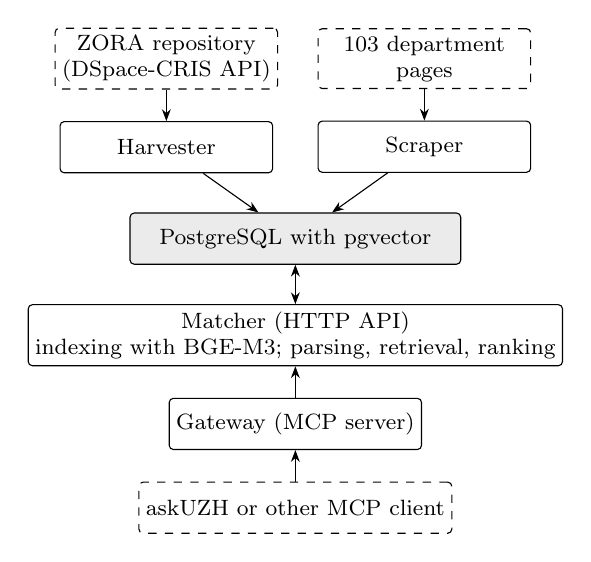
\begin{tikzpicture}[
  font=\footnotesize,
  box/.style={draw, rounded corners=1.5pt, align=center, inner sep=2.5pt,
              minimum height=6.5mm, minimum width=27mm},
  ext/.style={box, dashed},
  store/.style={box, fill=black!8, minimum width=42mm},
  arr/.style={-{Stealth[length=1.5mm]}, thin},
]
\node[ext] (zora) {ZORA repository\\(DSpace-CRIS API)};
\node[ext, right=5mm of zora] (web) {103 department\\pages};
\node[box, below=4mm of zora] (harv) {Harvester};
\node[box, below=4mm of web] (scr) {Scraper};
\node[store, below=5mm of $(harv.south)!0.5!(scr.south)$] (db) {PostgreSQL with pgvector};
\node[box, below=5mm of db, minimum width=59mm] (match)
  {Matcher (HTTP API)\\indexing with BGE-M3; parsing, retrieval, ranking};
\node[box, below=4mm of match] (gw) {Gateway (MCP server)};
\node[ext, below=4mm of gw] (client) {askUZH or other MCP client};
\draw[arr] (zora) -- (harv);
\draw[arr] (web) -- (scr);
\draw[arr] (harv) -- (db);
\draw[arr] (scr) -- (db);
\draw[arr, {Stealth[length=1.5mm]}-{Stealth[length=1.5mm]}] (match) -- (db);
\draw[arr] (client) -- (gw);
\draw[arr] (gw) -- (match);
\end{tikzpicture}
\caption{Components of \sys{}. Dashed boxes are external. The harvester and the scraper write source records, the matcher embeds them and answers queries, and the gateway exposes the matcher to assistants as MCP tools.}
\label{fig:arch}
\end{figure}

Figure~\ref{fig:arch} shows the components. Each runs as a separate process in its own container image.

\subsection{Data}

Publications come from ZORA through its DSpace-CRIS REST API. The harvester stores 214,756 records. The repository's authority links separate authors registered at UZH from external co-authors; 53,545 publications have at least one registered UZH author, and these name 2,942 distinct UZH authors. Incremental runs fetch newly accessioned records. Each run writes the raw responses to disk before touching the database, so a failed write can be replayed without querying ZORA again.

Thesis postings come from a scraper over 103 curated department pages. Each source has a declarative specification that locates listings and fields on the page, and extraction from these specifications is deterministic. A language model is used only to draft a specification when a source is added, which a person then approves, to summarise pages that describe application procedures, and as a fallback when a specification matches nothing, which is always flagged for review. Fetched pages are cached, so extraction can be rerun without contacting the sites, and every request carries a contact address. The index holds 695 postings, each with its named supervisors, the degree levels it is open to, and its status (open, pending, assigned or private).

\subsection{Indexing and Retrieval}

Both sources are embedded with BGE-M3~\cite{chen2024m3} (1024 dimensions, input truncated at 1024 tokens) and stored in PostgreSQL with pgvector~\cite{pgvector}. Retrieval uses cosine similarity over an HNSW index~\cite{malkov2020hnsw}. A content hash per document means that re-indexing embeds only new or changed records.

A query is first parsed into topics, an optional degree level and an optional department, by a rule-based parser or, when one is configured, by a language model. \sys{} then runs two retrievals, one over publications and one over postings. Degree level exists only on postings, so a single query filtered on ``master's thesis'' would drop every publication. Postings marked as assigned or private are excluded.

Each retrieved document is credited to people. A posting credits its named supervisors, and a publication credits its registered UZH authors. Only a publication with no registered UZH author credits all of its authors, so an external co-author of a UZH paper never receives credit. A person's score is the highest similarity among their credited documents, and the source of that document is kept with the score. By default, researchers registered at UZH rank above external researchers regardless of score.

\subsection{Resolving People Across Sources}\label{sec:identity}

The two sources write names differently. ZORA stores ``M\"uller, Anna'', while a department page may write ``Anna M\"uller'' or ``Prof.\ Dr.\ Anna M\"uller''. Grouped on the raw string, none of the 403 distinct supervisor names on postings matched any of the 2,942 UZH author names in ZORA.

\sys{} maps each name to a key formed from the first given name and the family name, after Unicode normalisation and with academic titles removed. Publications supply the reference keys, because ZORA's comma marks where a name divides, and names from postings are resolved against them. The rule is strict by design. The full first given name must agree, a family name alone never suffices, and a name that matches more than one reference key is left unmerged. We chose precision over recall because a false merge would present another person's publications to a student as evidence for a supervisor.

With this rule, 103 of the 403 supervisor names (25.6\%) resolve to a ZORA author, and we detected no false merge. Most of the rest cannot be reached by any rule on names. For 251 supervisors (62\%) ZORA holds no record at all, because thesis supervisors are often doctoral students, postdocs or staff of partner institutes. We also tried e-mail addresses as a veto, so that the same name with a different address would count as two people. The veto was wrong in five of the six cases where it applied, each time because one person used more than one address, and we dropped it. At the default depth of five results per source the resolution rarely changes a result: over five probe queries, none of the 25 returned matches combined the two sources.

\subsection{Abstention}\label{sec:abstain}

When nothing in the corpus fits a request, the system should say so rather than present the nearest researchers as a recommendation. \sys{} applies a threshold to the similarity score. If no candidate clears it, the written answer states that there is no strong match and names the closest candidate as a long shot, without calling a language model. The structured tool returns each score with its source, so that a calling assistant can apply the same rule.

We set the thresholds by measuring scores on the full index for five on-topic queries spread across faculties and four out-of-domain controls, everyday questions that no research group works on, such as how to proof sourdough. No document scored below 0.115 against any query, which is consistent with the anisotropy of contextual embeddings~\cite{ethayarajh2019contextual}: similarities fill a narrow positive band rather than the full range. Every control's best match scored below every on-topic query's best match, in both sources, so a threshold can separate the two classes. The two sources separate at different levels, however (Table~\ref{tab:bands}). A single threshold valid for both would have to lie in a band 0.022 wide, and any value in that band removes postings that are good matches. The likely cause is corpus size. Among 214,756 abstracts some document is nearly always close to a query, whereas the nearest of 695 short postings lies further away. \sys{} therefore uses one threshold per source, 0.57 for publications and 0.48 for postings. Nine queries establish the asymmetry but cannot fix the values, which we treat as a first calibration.

\begin{table}[t]
\caption{Best-match cosine similarity by query class on the full index, and the threshold applied per source.}
\label{tab:bands}
\small
\begin{tabular}{lccc}
\toprule
Source & Controls (highest) & On-topic (lowest) & Threshold \\
\midrule
Publications & 0.542 & 0.605 & 0.57 \\
Postings     & 0.431 & 0.564 & 0.48 \\
\bottomrule
\end{tabular}
\end{table}

\subsection{Serving and Integration}

Serving is split into two processes. The matcher holds the embedding model, the database connection and the language-model client, and exposes an HTTP API for matching, recommendation and index status. The gateway is a thin MCP server over streamable HTTP with two tools. \texttt{find\_researchers} returns the ranked researchers and their evidence as structured data, and \texttt{recommend\_supervisors} returns a short written answer. The deployment environment required this split. An earlier gateway ran retrieval in-process and needed about 3.6\,GiB of memory in a namespace with a 4\,GiB quota; the gateway now holds no model and no database connection.

When \sys{} writes the answer itself, the language model sees only the retrieved candidates and their listed work. It is instructed to name no one else and to say plainly when a candidate fits only in part. An early run showed that the prompt must also omit information the system does not have. Given a line stating that a researcher had no open position in our data, the model wrote that the researcher was not accepting students, which the data cannot support. The prompt now leaves out the posting line when there is none.

\section{Evaluation}\label{sec:eval}

\subsection{Benchmark}

No collection of real student queries with judged supervisors exists for UZH, so we generated one. We sampled 150 supervisors with between 3 and 20 publications and a verified repository identity, and 150 postings. KeyBERT~\cite{grootendorst2020keybert}, with a multilingual sentence encoder~\cite{reimers2020multilingual}, extracted keywords from each supervisor's publications and from the text of each posting. A language model then phrased 2, 4 or 8 of these keywords as a student's request. This gives three levels of detail per target and 900 queries in total. \TODO{name the model that phrased the queries; the benchmark manifest does not record it} The supervisors behind the source documents are the gold answer. We report Hit@$k$, the fraction of queries whose target appears in the top $k$, and mean reciprocal rank (MRR)~\cite{voorhees1999trec8} over the top ten results, with a miss counted as zero.

The benchmark has a known bias. Each query is derived from its target's own documents, so it tests whether \sys{} recovers the author of a text, and the queries share more vocabulary with their sources than a student's request would. Each query also has a single gold answer, so another researcher who would supervise well counts as a miss. Generated test collections inherit biases from the models that produced them~\cite{rahmani2024synthetic}. We therefore read the results as a measure of retrieval and crediting, not of recommendation quality, which needs judgements from students and supervisors.

\subsection{Results}

\begin{table}[t]
\caption{Ranking results on 900 generated queries. Rows below the first break results down by source, by number of keywords in the query, and, for publication queries, by the target's publication count.}
\label{tab:main}
\small
\begin{tabular}{lrcccc}
\toprule
Subset & $n$ & Hit@1 & Hit@5 & Hit@10 & MRR \\
\midrule
All queries          & 900 & .660 & .832 & .848 & .730 \\
\midrule
Publication queries  & 450 & .529 & .751 & .762 & .619 \\
Posting queries      & 450 & .791 & .913 & .933 & .841 \\
\midrule
2 keywords           & 300 & .593 & .817 & .837 & .684 \\
4 keywords           & 300 & .663 & .810 & .833 & .724 \\
8 keywords           & 300 & .723 & .870 & .873 & .782 \\
\midrule
Publications, $\geq$10 & 267 & .491 & .738 & .749 & .590 \\
Publications, $<$10    & 183 & .585 & .770 & .781 & .661 \\
\bottomrule
\end{tabular}
\end{table}

Table~\ref{tab:main} gives the results. The target is ranked first for 66.0\% of queries and appears in the top five for 83.2\% (MRR 0.730). Queries built from postings score higher than queries built from publications (MRR 0.841 against 0.619). A posting names its supervisor directly and sits in an index of 695 documents, whereas a publication query must single out one author among 214,756 records, each of which may credit several UZH co-authors. MRR rises with the number of keywords (0.684, 0.724 and 0.782 for 2, 4 and 8), as expected when queries echo their source text.

One result runs against intuition. Among publication queries, supervisors with ten or more publications are found less often than those with fewer (MRR 0.590 against 0.661). Prolific researchers have more co-authors, and a publication credits all its UZH authors, so a prolific researcher may share their best documents with colleagues who then rank above them. We have not tested this explanation.

\subsection{Specificity}

We asked whether the ranking separates a researcher's specialisation from the surrounding field. For eight supervisors we issued three queries each. One was generated from their own work, one named an adjacent specialisation they do not work on, and one named the general field. For a researcher in protein design, for instance, the adjacent query might name drug discovery and the general query biochemistry. A supervisor should rank higher for their own specialisation than for either of the others. This held for four of the eight. Two supervisors were absent from the top ten for all three queries, which is a failure of recall rather than of specificity. For the other two the order was reversed; one ranked third for the general field and sixth for the adjacent topic, but outside the top ten for their own. Eight cases illustrate rather than measure, but they suggest that the embedding often matches the neighbourhood of a topic rather than the specialisation.

\subsection{Student Background}

\begin{table}[t]
\caption{Adding information about the student to the query (100 supervisors).}
\label{tab:ablation}
\small
\begin{tabular}{lccc}
\toprule
Query content & Hit@1 & Hit@5 & MRR \\
\midrule
Topic only                     & .450 & .730 & .563 \\
Topic + study programme        & .470 & .670 & .559 \\
Topic + background             & .410 & .680 & .527 \\
Topic + programme + background & .410 & .670 & .521 \\
\bottomrule
\end{tabular}
\end{table}

Students often describe more than a topic, adding their degree programme, the courses they have taken or earlier projects. We tested whether this helps. For 100 supervisors we generated the same topic query in four variants (Table~\ref{tab:ablation}), and none improved on the topic alone. MRR fell from 0.563 to 0.559 with the study programme, 0.527 with the background and 0.521 with both, and Hit@5 fell from 0.730 to between 0.670 and 0.680. We have not tested these differences for significance, and at this sample size the smallest may be noise. The direction matches how retrieval works. The whole query becomes one vector, and text about the student moves that vector away from documents about the topic. Context of this kind is more likely to help as a filter or re-ranking signal than as part of the embedded query.

\section{Demonstration}\label{sec:demo}

The demonstration follows a student through one session. It runs through an MCP client connected to the gateway, so that visitors see each tool call as the assistant makes it; the same session also runs from the command line.

The student first describes an interest in their own words, for example a master's thesis on misinformation detection with language models. The assistant calls \texttt{find\_researchers}, and visitors see the structured result. It lists researchers in rank order, each with a department, a score, the source of that score, and the publications and postings behind the match, linked to ZORA and to the department page. Adding ``master's thesis'' to the request restricts postings to those open at that level and leaves publications in place.

Two contrasts show the design decisions at work. A researcher recommended for their publications appears next to one recommended for an open thesis posting, and the source field shows why each is there. A request that no research group covers, such as the sourdough control from Section~\ref{sec:abstain}, scores below both thresholds, and the written answer reports that there is no strong match instead of presenting the nearest researcher as a fit. Visitors can also set the written answer from \texttt{recommend\_supervisors} beside the structured list and check that every person it names appears in the list. \TODO{screenshot of one session; decide how to show real researchers' names, which are personal data}

\section{Conclusion}

\sys{} recommends supervisors from a university's own publication records and thesis postings. It credits evidence to people across both sources with a deliberately strict rule and abstains using thresholds set per source from measurements on the full index. On generated queries it finds the target supervisor in the top five for 83.2\% of cases, but it often fails to separate a specialisation from its field, and extra context about the student lowers accuracy.

Several parts remain open. Ranking uses only the best similarity score, although publication counts, recency and open postings are available. Identity resolution reaches a quarter of supervisors, and the researcher profiles already scraped from department pages are a likely source for many of the rest. The thresholds rest on nine queries and need a larger calibration set, and the integration into askUZH is not yet deployed. The largest gap is in the evaluation. The benchmark measures retrieval against generated queries, and whether the recommendations help students is a question for the study with students and supervisors that we are preparing.

\begin{acks}
\TODO{thank the supervisors and the askUZH team by name}
\end{acks}

\bibliographystyle{ACM-Reference-Format}
\bibliography{refs}

\end{document}
